%----------------------------------------------------------------------------------------
%	CHAPTER 2 // Starburst Eye Tracking Algorithm
%----------------------------------------------------------------------------------------
\chapterimage{single_eye.jpg}
\chapter{Starburst Eye Tracking Algorithm}
\label{ch_starburst}
As proposed in the previous chapters that we rely on 2 different approaches to provide a new user experience; Eye-tracking, and gesture recognition. Through this chapter we will go through the details of our eye-tracking module, what algorithms we used, problems we faced, and workarounds to that problems.

\begin{eBox}
In this chapter we will use the \: \: \begin{tikzpicture}[overlay]
\node[draw=ocre!60,line width=1pt,circle,fill=ocre!25,font=\sffamily\bfseries,inner sep=2pt,outer sep=0pt] at (0pt,3pt){\textcolor{ocre}{R}};\end{tikzpicture}  \: \: mark to indicate parts that describe our implementation and modifications to the original Starburst algorithm.
\end{eBox}

\section{Starburst}\index{Starburst}
In the first version of our eye-tracking module we went for implementing the Starburst \cite{starburst}.The Starburst eye-tracking algorithm combines feature-based and model-based approaches to achieve a good trade off between run-time performance and accuracy for dark-pupil infrared illumination. The goal of the algorithm is to extract the location of the pupil center and estimate point of gaze using a homography matrix. As figure \ref{fig:starburst_overview} shows, the algorithm begins by locating and removing the corneal reflection from the image. Then the pupil edge points are located using an iterative feature-based technique. An ellipse is fitted to a subset of the detected edge points using the Random Sample Consensus (RANSAC) paradigm. The best fitting parameters from this feature-based approach are then used to initialize a local model-based search for the ellipse  parameters that maximize the fit to the image data.


\begin{figure*}[h]
\begin{dBox}
\centering
	\mbox{
		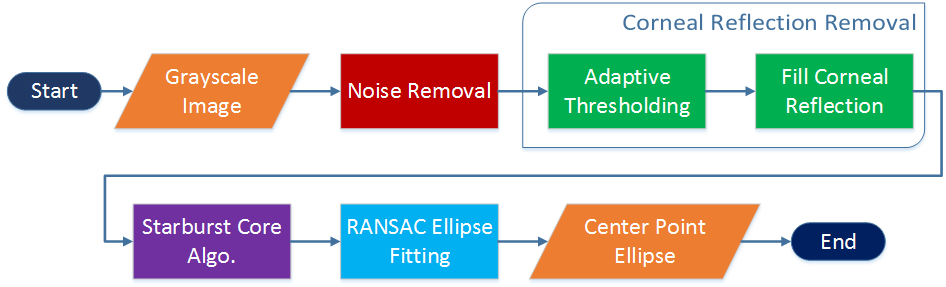
\includegraphics[width=\textwidth]{./Pictures/starburst/Starburst_overview.png}
	}
   \caption{Overview of MIRT Algorithm \label{fig:starburst_overview} }   
\end{dBox}   
\end{figure*}


\section{Noise Reduction}\index{Noise Reduction}
The Starburst algorithms deals with two types of noise that are commonly encountered in any low cost head-mounted eye-tracker. The two types of noise are the shot noise and the line noise. Shot noise is reduced by applying a $5x5$ Gaussian filter with a standard deviation of $2$ pixels. Line noise is reduced by applying a normalization factor is applied line by line to shift the mean intensity of the line to the running average derived from previous frames. The following modeling describes the process of line noise reduction as proposed in Startburst \cite{starburst}.

\begin{dBox}
\centering
	\begin{equation}
	C(i,l) = \beta \bar I  (i,l) + (1 - \beta) C(i-1, l)
	\end{equation}
\end{dBox}

Where $C(i,l)$ is the normalization factor, $I(i,l)$ is the average line intensity and $B = 0.2$. Keep in consideration that the noise reduction step is optional and can be deactivated if the used camera is capable of capturing less noisy images. \bigskip

\begin{our}
In our implementation we didn't do any modifications to the noise reduction module. We implemented this module as described in the Starburst algorithm \cite{starburst}. Note that using head-mounted camera in our system doesn't require noise reduction, so this module is deactivated at runtime.
\end{our}


\section{Corneal Reflection}\index{Corneal Reflection}
\subsection{Detection and Localization}\index{Detection and Localization}

The corneal reflection corresponds to one of the brightest regions in the eye image. Thus the corneal reflection can be obtained through thresholding. However, a constant threshold across observers and even within observers is not optimal. Therefore we use an adaptive thresholding technique in each frame to localize the corneal reflection. \bigskip

One of the heuristics adopted by the Starburst algorithm is that cornea extends approximately to the limbus, so the search space for the cornea can be limited with a square region of interest by half width of $h = 150$ which makes sense. Other heuristic which we believe is the core of the corneal reflection detection is that the corneal reflection is the largest and the brightest candidate region in the region of interest, as other specular reflections tend to be quite small and located off the cornea as well as near the corner of the image where the eye lids meet. \bigskip

At first the input (gray scale) frame is converted to binary form, only values above the maximum threshold are taken as corneal reflection candidates. Then the ratio between the area of the largest candidate to the average area of other regions is calculated as the threshold is lowered. A notable observation is that the intensity of the corneal reflection monotonically decreases towards the edges.\bigskip

At the beginning the ratio between  largest candidate area and average area of other candidates will increase since the corneal reflection will grow in size faster than other areas. As the threshold is decreased the ratio will begin to drop because the false candidates are becoming of significant size compared to the corneal reflection. The optimal threshold is the threshold that generates the hight ratio. The largest candidate using the optimal threshold is considered the corneal reflection with the geometric center $(c_{x}, c_{y})$. \bigskip

In the Starburst algorithm the corneal reflection intensity profile is assumed to follow a bivariate Gaussian distribution. Full extent of the corneal reflection is obtained by relating the the radius $r$ where the average decline in intensity is maximal to the radius with maximal decline for a Gaussian (i.e. a radius of one standard deviation). To capture 99\% of the corneal reflection profile use $2.5r$. Where $r$ is computed through a gradient decent search that minimizes:


\begin{dBox}
	\begin{equation}
		\frac{ \int I ( r + \delta, x_{c}, y_{c}, \theta ) d\theta }{ \int I ( r - \delta, x_{c}, y_{c}, \theta ) d\theta}
	\end{equation}
\end{dBox}

where $\delta = 1$ and $I(r, x, y, \theta)$ is the pixel intensity at angle $\theta$ on the contour of a circle defined by the parameters $r$, $x$, and $y$. The search is initialized with $r = \sqrt{area/\pi}$, where area is the number of pixels in the thresholded region. The search converges rapidly.\bigskip

\begin{our}
In our implementation we used a simplified version for corneal reflection detection procedure described by the Starburst algorithm. First step we convert the input gray scale image to binary form. Then we perform adaptive thresholding until we find the optimal threshold (which generates the highest ratio) as described in the original algorithm. Next we estimate the the center of corneal reflection region. Till now no differences from the original algorithm. The main difference is that we assume that the corneal reflection is circular and hence we find the radius from the area of circle relation $r = \sqrt{ area_{max} / \pi }$.
\end{our}

\subsection{Removal}\index{Removal}
Original Starburst algorithm uses radial interpolation to remove the corneal reflection. First, the central pixel of the identified corneal reflection region is set to the average of the intensities along the contour of the region. Then for each pixel between the center and the contour, the pixel intensity is determined via linear interpolation. \bigskip

\begin{our}
Our implementation of the corneal reflection removal is different to the original algorithm, we assume that the corneal reflection is circular and hence we fill a circular region in the image with an estimation of the pupil intensity. The pupil intensity is estimated by averaging the intensity along the ring that encapsulates the corneal reflection and is $d$ pixels larger than corneal reflection radius, where $d$ is set to 10 pixels.
\end{our}


\section{Starburst Core Algorithm}\index{Starburst Core Algorithm}

Unlike most of feature based eye tracking approaches that apply edge detection to the entire image, Starburst algorithm detects edges along a limited number of rays that extend from a central best guess of the pupil center. These rays can be seen in Figure \ref{pupil_rays}. This method takes advantage of the high-contrast elliptical profile of the pupil contour present in images taken using the dark-pupil technique. Algorithm pseudo code is shown in algorithm \ref{starburst_psuedo}. \bigskip


\begin{algorithm}
\begin{dBox}
	\caption{Starburst Original Algorithm} \label{starburst_psuedo}
	\begin{algorithmic}[1]
		\Require{Eye image - corneal reflection removed, Best guess of pupil center}
		\Ensure {Set of feature points}
		\Procedure{Starburst}{}
			\Repeat  
				\vspace{1em}	
				\State \emph{Stage 1:}
					\State Follow rays extending from the starting point
					\State Calculate intensity derivative at each point
					\If {$derivative > threshold$} 
						\State Place feature point
						\State Halt marching along ray
					\EndIf		
				\vspace{1em}	
				\State \emph{Stage 2:}
					\ForAll {feature points detected in Stage 1}
						\State March along rays returning towards the start point
						\State Calculate intensity derivative at each point
						\If {$derivative > threshold$} 
							\State Place feature point
							\State Halt marching along ray
						\EndIf		
					\EndFor
					\vspace{.3em}			
					\State Starting point = geometric center of feature points
			\vspace{1em}							
			\Until{starting point converges}
		\EndProcedure	
	\end{algorithmic}
\end{dBox}	
\end{algorithm}

For each frame a location is chosen that represent the best guess of the pupil center in this frame. The best guess at the first frame is chosen to be the center of the image, best guess at frame $i$ are set to be the center of the pupil detected in the previous frame (frame $i-1$).  Next, the derivatives $\vartriangle$ along the $N = 18$ rays, extending radially away from this starting point, are independently evaluated pixel by pixel until a threshold $\phi = 20$ is exceeded. Since Starburst uses a dark-pupil technique, only positive derivatives (increasing intensity as the ray extends) are considered. When the value of the derivative along the line exceeds the threshold a features point (pupil edge candidate point) is marked, and the processing along this line is halted. If the processing along a line reached borders of the image no feature point is marked. Example of the candidate feature points and corresponding rays are shown at figure \ref{fig:starburst_example}. \bigskip


\begin{figure*}[]
\begin{dBox}
\centering
  \mbox{
      \subfigure[Stage 1 rays]{
            \label{fig:stage_1}
            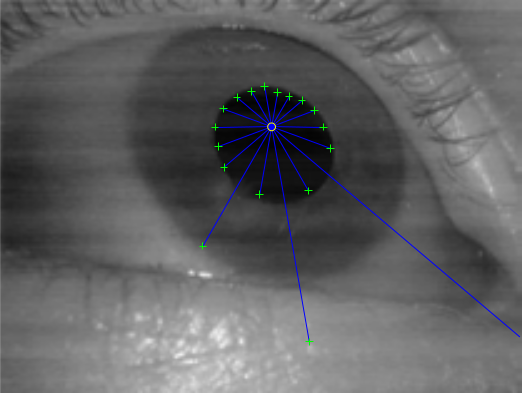
\includegraphics[width=.31\textwidth]{./Pictures/starburst/3a.png}
        }
        \subfigure[Stage 2 inlier point]{
           \label{fig:stage_2_inlier}
           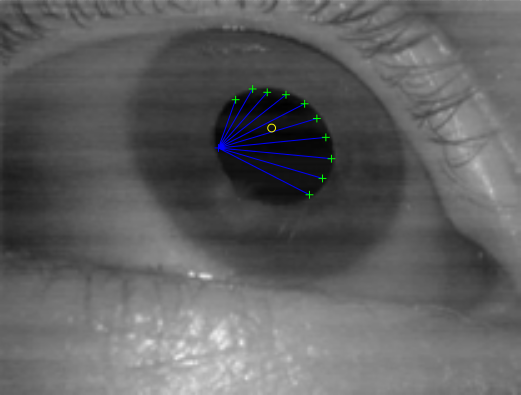
\includegraphics[width=.31\textwidth]{./Pictures/starburst/3b.png}
        }
        \subfigure[Stage 2 outlier point]{
            \label{fig:stage_2_outlier}
            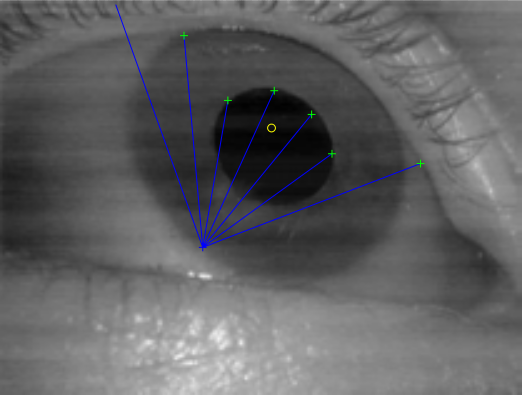
\includegraphics[width=.31\textwidth]{./Pictures/starburst/3c.png}
       }
   }
   \caption{Visualization of Starburst stage 1 and stage 2 feature point detection procedure \label{fig:starburst_example} }   
\end{dBox}   
\end{figure*}

For every feature point obtained the above described algorithm is repeated with a minor modification. Search rays are limited to $\gamma = \pm 50$ degrees from the original ray that originally produced the feature point. This procedure tends to increase the ratio of the number of feature points on the pupil contour over the number of feature points not on the pupil contour. If the pivot feature point lies on the pupil contour then the rays around the original ray will result in feature points that also lie on the opposite half of the pupil contour. On the other hand if the original feature point is not on the pupil contour, then limiting the search space will cut down the number of feature point that doesn't lie on the pupil contour. One important note to take into consideration is that the number of rays in this step is only 10 (5 on each side of the original ray). Figure \ref{fig:starburst_stage2_example} shows the two cases described above. \bigskip



\begin{figure*}[h]
\begin{dBox}
\centering
  \mbox{
        \subfigure[Stage 2 inlier point]{
           \label{fig:stage_2_inlier_p}
           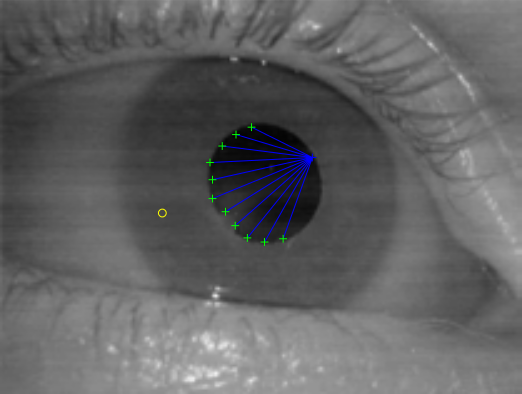
\includegraphics[width=.31\textwidth]{./Pictures/starburst/4b.png}
        }
        \subfigure[Stage 2 outlier point]{
            \label{fig:stage_2_outlier_p}
            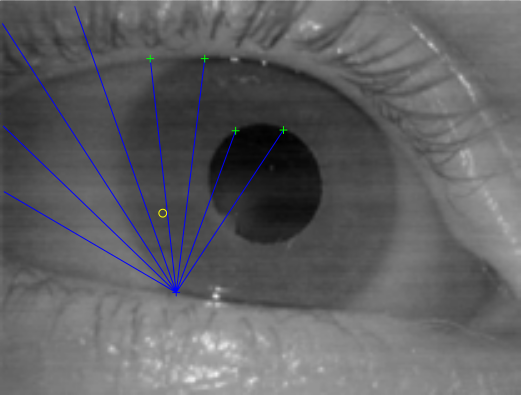
\includegraphics[width=.31\textwidth]{./Pictures/starburst/4c.png}
       }
   }
   \caption{Visualization of Starburst stage 2 feature point detection procedure \label{fig:starburst_stage2_example} }   
\end{dBox}   
\end{figure*}

Using the two stage feature detection process improves the robustness of the method to poor initial guesses for the starting point. However, the feature points tend to bias to the side of the pupil contour nearest the initialization point. Although another iteration of the ray process would minimize this bias, the computational burden grows exponentially with each iteration and thus would be an inefficient strategy. \bigskip

Fitting an ellipse to the set of biased feature points will induce significant error into fit. A good strategy to eliminate the bias is to iterate the recently described procedure, with each time computing the average of the detected feature points to be the new estimated center of the pupil for the next iteration. The iterating process is halted when the estimated pupil center between two successive iteration is less than $d = 10$ pixels. Starburst paper mention that if guess is a good estimate of the pupil center, only a single iteration is required. When the initial estimate is not good, typically only a few iterations ($< 5$) are required for convergence. If convergence is not reached within $i = 10 $iterations, as occurs sometimes during a blink when no pupil is visible, the algorithm halts and begins processing the next frame. \bigskip

\begin{our}
In out implementation of this module we sticked to the exact Startburst algorithm described in the paper.
\end{our}


\section{Ellipse Fitting}{Ellipse Fitting}
Given a set of feature points, the function of this module is to find best fitting ellipse.  Most of algorithms use least-squares ellipse fitting including all feature points (e.g. see \cite{least_squares}). Using all points to estimate an ellipse results in significant error that strongly affect the accuracy. Notice that a few feature points not on the pupil contour dramatically reduces the quality of the fit to an unacceptable level.  \bigskip

To address this issue Starburst uses Random Sample Consensus (RANSAC) paradigm for model fitting \cite{ransac}. Starburst paper claims that Starburst is the first algorithm that uses RANSAC in the context of eye-tracking. RANSAC is an effective technique for model fitting in the presence of a large but unknown percentage of outliers in a measurement sample. A basic assumption is that the data  consists of "inliers", i.e., data whose distribution can be explained by some set of model parameters, though may be subject to noise, and "outliers" which are data that do not fit the model. In our application inliers are feature points that lie on the pupil contour, while outliers are feature points that belong to other contours other than the pupil contour. Least-squares approaches assumes that all sample points fit the model and hence, uses all the sample points to estimate the model. On the other hand RANSAC is an iterative method to estimate parameters of a mathematical model from a set of observed data which contains outliers. General outline of RANSAC technique is shown at algorithm \ref{ransac_outline}. \bigskip

\begin{algorithm}
\begin{dBox}
	\caption{General RANSAC Procedure} \label{ransac_outline}
	\begin{algorithmic}[1]
		\Procedure{RANSAC}{}
		 \While{$i < N$}
			\State Draw $s$ points uniformly at random
			\State Fit model to these $s$ points
			\State Find inliers to this model among the remaining points (points whose error $ < t$)
			\State If there are $d$ or more inliers, accept the model and refit using all inliers	
		\EndWhile	
		\EndProcedure	
	\end{algorithmic}
\end{dBox}	
\end{algorithm}


The output of the two stage feature detection process may result in very few outliers in some cases, while in other cases outlier prevail. Using the RANSAC technique increase the ability of the system to do robust estimation of the model (ellipse) parameters. The following procedure is repeated $R$ times. First, five samples are randomly drawn from the set of feature set obtained by the previous module.  Singular Value Decomposition (SVD) on the conic constraint matrix generated with normalized feature-point coordinates \cite{multipleViewGeom} is used to find the parameters of the ellipse that perfectly fit these five points. Then, the number of candidate feature points in the data set that agree with this model (i.e. the inliers) are counted. Inliers are those sample points for which the algebraic distance to the ellipse is less than some threshold $t$. \bigskip

\begin{our}
Our implementation of this stage differs a bit from the implementation of the original Starburst. We draw 5 samples from the detected feature set, then we compute the best fit ellipse using Fitzgibbon's algorithm \cite{fitzgibbon96} which is implemented in OpenCV. Finally we evaluate the error between the estimated model and all feature points and count inliers / outliers. Algorithm \ref{our_ransac_outline} summarizes how we use RANSAC in our system. \bigskip

\begin{algorithm}
\begin{dBox}
	\caption{Our RANSAC Procedure} \label{our_ransac_outline}
	\begin{algorithmic}[1]
		\Procedure{RANSAC}{}
		 \While{$i < N$}
			\State Draw $s$ points uniformly at random
			\State Fit ellipse model to these $s$ points
			\State Find inliers to this ellipse (points whose algebraic error $ < t$)
			\State If there are $d$ or more inliers, accept the ellipse and refit using all inliers	
		\EndWhile	
		\EndProcedure	
	\end{algorithmic}
\end{dBox}	
\end{algorithm}


As a matter of fact we tried different approaches in our implementation, at first we tried to implement the same approach mentioned in the Starburst paper. However finding the SVD of the parameter matrix using OpenCV SVD didn't produce consistent results because the calculated eigen vectors / values were not correct. Some books like \cite{practicalOpenCV} addressed this issue and suggested using Eigen mathematics library \cite{eigenweb} to find the eigen values/vector. In our application we couldn't benefit from this solution since, Eigen library is only available in C++ while the user end if our application is in Java (Android user end).
\end{our}

\subsection{Estimation of Number of Iterations $R$}\index{Number of Iterations}
Starbusrt algorithm assumes that the average error variance of the feature detector is approximately one pixel and that this error is distributed as a Gaussian with zero mean. Thus to obtain a 95\% probability that a sample is correctly classified as an inlier, the threshold should be derived from a $\chi^{2}$ distribution with one degree of freedom \cite{multipleViewGeom}. This results in a threshold distance of $t = 1.98$ pixels. \bigskip

The parameter R (the number of iterations), however, can be determined from a theoretical result. Let p be the probability that the RANSAC algorithm in some iteration selects only inliers from the input data set when it chooses the $s$ points from which the model parameters are estimated. When this happens, the resulting model is likely to be useful so $p$ gives the probability that the algorithm produces a useful result. Let $w$ be the probability of choosing an inlier each time a single point is selected, that is, 
\begin{dBox}
	$$ w = \frac{number \: of \: inliers \: in \: data}{number \: of \: points \: in \: data} $$
\end{dBox}
it can be proven that 
\begin{dBox}
\begin{equation}
		R = \frac{log(1-p)}{log(1-w^{5})}
\end{equation}
\end{dBox}

\section{Homographic Mapping and Calibration}\index{Homographic Mapping and Calibration}
In order to calculate the point of gaze of the user in the scene image, a mapping between locations in the scene image and an eye-position measure must be determined. The typical way to determine the mapping is via a calibration process. During calibration, the user is required to look at a number of scene points for which the positions in the scene image are known. At each position the eye-position $\vec{e} = (x_{e} ,\: y_{e},\: 1)$ and the scene position $\vec{s} = (x_{s},\: y_{s},\: 1)$ is measured. The mapping is generated using the $3x3$ homography matrix which has 8 degrees of freedoms. Each point (map from scene to eye) produces 2 independent equations. Hence four mapping points are needed to compute the entries of the homography matrix up to scale \cite{heuristic}. \bigskip

\begin{our}
In our implementation we use the OpenCV \textit{findHomography} procedure to find the homography matrix. Given a set of points in image coordinates and corresponding set of points in the eye coordinates, \textit{findHomography} finds a perspective transformation between two coordinate systems.
\end{our}

Once this mapping is determined the user’s point of gaze in the scene for any frame can be established
as $\vec{s} = H \vec{e}$.
